\chapter{Resultados} \label{resultados}

A API pode ser encontrada em funcionamento em um ambiente de testes no link \href{http://bit.ly/tcc-pdf}{http://bit.ly/tcc-pdf}. Suas funcionalidades de leitura encontram-se livres para serem acessadas, porém as funcionalidades que alterem o estado do banco de dados estão restritas aos usuários cadastrados. Apesar de estar em funcionamento e livre para ser acessada, este é apenas um ambiente de testes, e sua hospedagem no servidor do Núcleo de Biologia Computacional e Gestão de Informações Biotecnológicas (NBCGIB) está sendo configurada.

Para o controle destas utilidades existem duas camadas de segurança. 
A camada de chave de API, apresentada na \textbf{Figura \ref{swaggerAPIKey}} assegura que somente os administradores do sistema, em posse da chave, possam registrar e remover usuários da API.

\begin{figure}[H]
\centering
\captionsetup{justification   = raggedright,
              singlelinecheck = false}
\caption{Autorização por Chave de API - Swagger UI}\label{swaggerAPIKey}
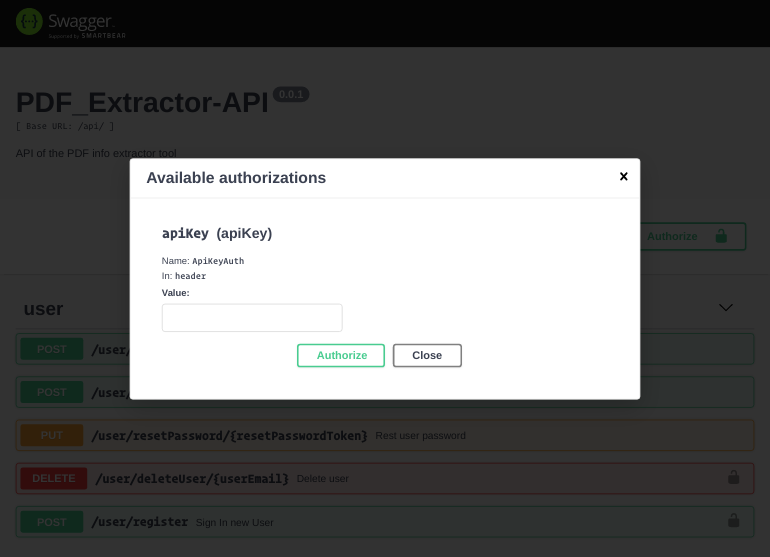
\includegraphics[width=0.9\textwidth]{figs/swaggerAPIKey.png}
\footnotesize Fonte: Autoria Própria
\end{figure}

A camada de usuário garante a integridade do sistema, pois esta impede que usuários não autenticados tenham acesso a funcionalidades que alterem o estado do banco de dados. Na \textbf{Figura \ref{swaggerLogin}} é possível ver o método de login, e suas possíveis respostas.

\begin{figure}[H]
\centering
\captionsetup{justification   = raggedright,
              singlelinecheck = false}
\caption{Login de Usuário - Swagger UI}\label{swaggerLogin}
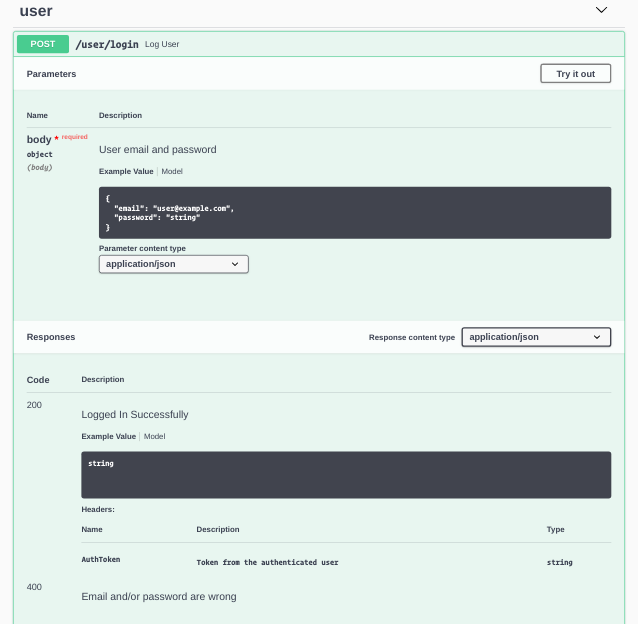
\includegraphics[width=1\textwidth]{figs/swaggerLogin.png}
\footnotesize Fonte: Autoria Própria
\end{figure}

Para o categoria de funções do usuário, assegurando o acesso e contendo funcionalidades necessárias para o administrador do sistema apresenta as seguintes funcionalidades:

\begin{itemize}
    \item \textbf{Login}: Como explicado no tópico \ref{apiDev}, recebe e-mail e senha e retorna um \textit{token} caso a autenticação o ocorra com sucesso.
    
    \item \textbf{Senha Esquecida}: Recebe o e-mail do usuário, sendo ele valido, é disparado um e-mail contendo um identificador único para a recuperação da senha.
    
    \item \textbf{Resetar Senha}: Continuando o fluxo da função anterior, recebe o identificador e uma nova senha, caso sejam válidos, a nova senha é atribuída ao usuário.
    
    \item \textbf{Remover Usuário}: Recebe um e-mail de usuário e a chave de API, caso sejam válidos, o usuário correspondente a aquele e-mail é desativado.
    
    \item \textbf{Registrar Usuário}: Recebe e-mail e senha do usuário a ser cadastrado. Também deve ser enviada a chave de API para validação do administrador. A coleção de usuários, no banco de dados, se encontra livre de \textit{schema} devido aos diferentes tipos de usuários. 
\end{itemize}

Para que o usuário tenha controle das configurações do conteúdo a ser extraído, foi criada a seção de Extração:

\begin{itemize}
    \item \textbf{Registrar Parâmetros}: Conforme explicado anteriormente no tópico \ref{apiDev}, esta requisição recebe um objeto JSON, com as informações necessárias para realizar um extração, e o \textit{token} de usuário, como pode ser observado na \textbf{Figura \ref{swaggerExtractParam}}. Este objeto é salvo no banco de dados e utilizado ao realizar extrações.
    
    \item \textbf{Parâmetros Registrados}: Realiza uma consulta no banco de dados e retorna um objeto JSON com um vetor de parâmetros que já estão registrados.
    
    \item \textbf{Remover Parâmetro}: Recebe um ID de parâmetro e o \textit{token} de usuário, sendo válidos, o parâmetro é removido do banco de dados.
\end{itemize}

\begin{figure}[H]
\centering
\captionsetup{justification   = raggedright,
              singlelinecheck = false}
\caption{Parâmetros de Extração - Swagger UI}\label{swaggerExtractParam}
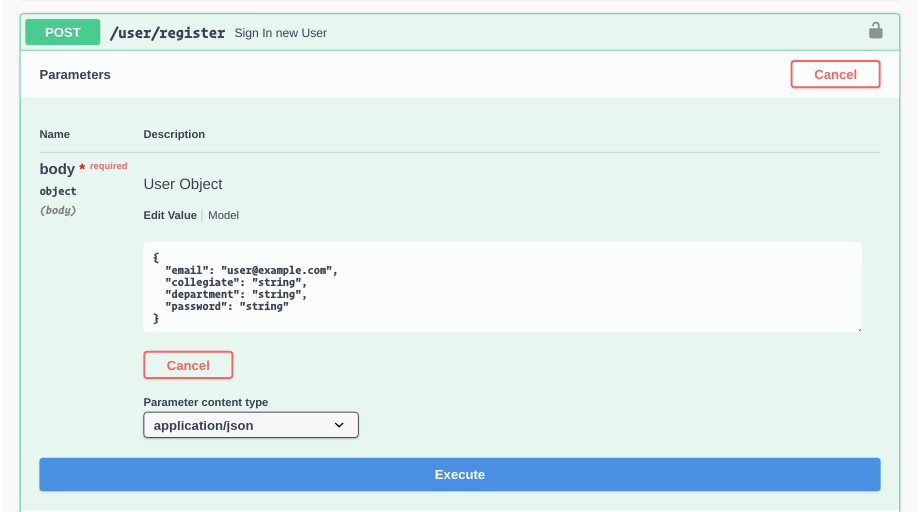
\includegraphics[width=1\textwidth]{figs/SwaggerUIExample.png}
\footnotesize Fonte: Autoria Própria
\end{figure}

Em relação a informação já extraída, são entregues as seguintes funcionalidades:

\begin{itemize}
    \item \textbf{Informações Extraídas}: Consulta no banco de dados todas as informações extraídas e as retorna em um vetor de objetos JSON correspondente a cada arquivo, contendo as informações que foram extraídas de tal.
    
    \item \textbf{Remover Informação Extraída}: Recebe o ID correspondente a um objeto de informações extraídas, e um \textit{token} de usuário, sendo válido, remove o objeto do banco de dados.
\end{itemize}

Por fim há a função responsável por receber um arquivo, o \textit{token} de usuário e a identificação do arquivo, como pode ser visto na \textbf{Figura \ref{swaggerUploadFile}}. Ao ser recebido, são buscados os parâmetros que possuem o mesmo valor do arquivo enviado no campo \textit{docType}, e assim serão extraídas as informações para cada parâmetro definido. A requisição é respondida com um objeto JSON contendo todas as informações extraídas, em caso de sucesso.

\begin{figure}[H]
\centering
\captionsetup{justification   = raggedright,
              singlelinecheck = false}
\caption{Envio de Arquivo - Swagger UI}\label{swaggerUploadFile}
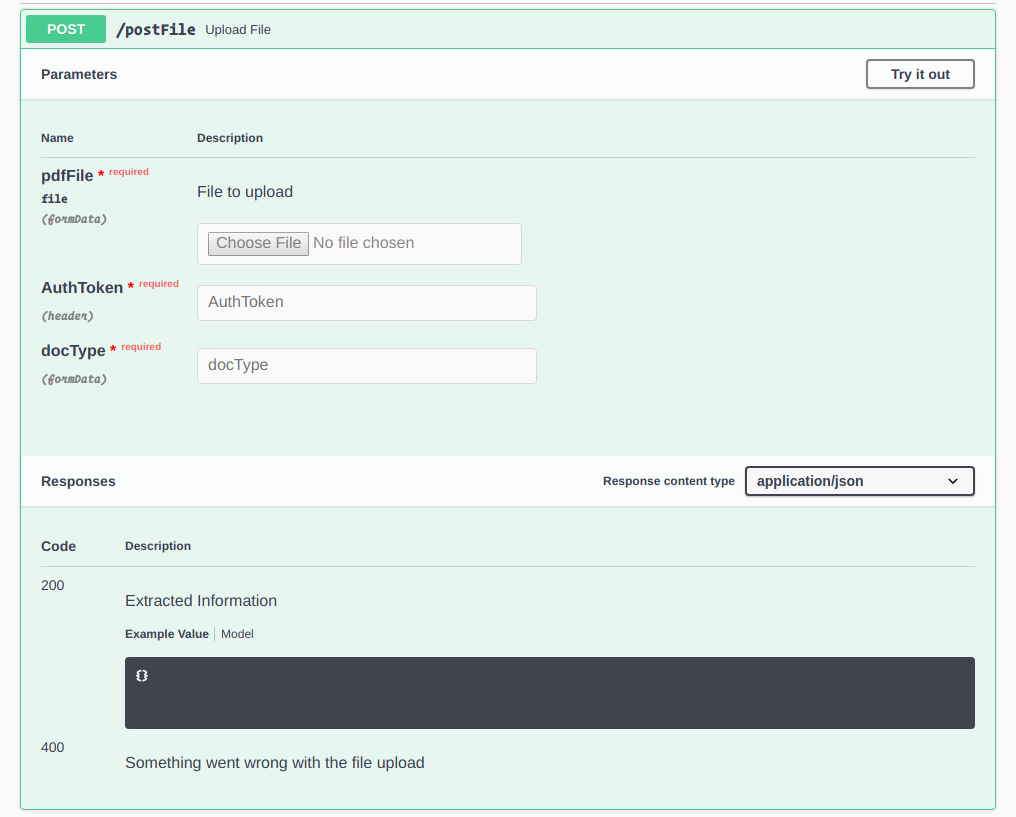
\includegraphics[width=1\textwidth]{figs/swaggerUploadFile.png}
\footnotesize Fonte: Autoria Própria
\end{figure}

Como pode ser notado nas imagens apresentadas neste capitulo, toda a API está documentada e pronta para uso na interface do Swagger, que pode ser encontrada no caminho \textit{/api/docs} (partindo do endereço raiz da aplicação). Neste endereço é possível fazer a utilização da API e ter o entendimento do que cada função faz e o que deve ser retornado.

No curso de Ciência da Computação da UESC há um projeto em desenvolvimento para a criação de uma rede de egressos. Sendo o trabalho de conclusão de curso aprovado, este é o primeiro passo para o aluno se tornar um egresso. Desta forma foi notado que há uma demanda por informações referentes aos egressos que podem ser encontradas no arquivo PDF do trabalho, assim é possível extrair um espécie de ficha do egresso contendo nome do autor, orientador, título do trabalho, palavras-chave e resumo.

Com esta demanda e a necessidade de por a prova a API, foi desenvolvida uma aplicação \textit{front-end} para a utilização do colegiado do curso. 

% Conforme apresentado na figura 12, todas as funcionalidades de usuário da API estão apresentadas nesta tela login

% Conforme apresentado na \textbf{Figura \ref{login}}, todas as funcionalidades, pertinentes a usuário, estão ligadas as funções da API. Esta tela representa a página de login por onde o colegiado deve acessar o sistema.

% Utilizando a chave de API foi criada uma conta de usuário para o colegiado. Na \textbf{Figura \ref{login}} a tela de login no sistema do colegiado é apresentada. Todas as funcionalidades de usuário estão em comunicação com as funções da API.

% \begin{figure}[H]
% \centering
% \captionsetup{justification   = raggedright,
%               singlelinecheck = false}
% \caption{Login - Sistema de Extração de dados de TCC}\label{login}
% 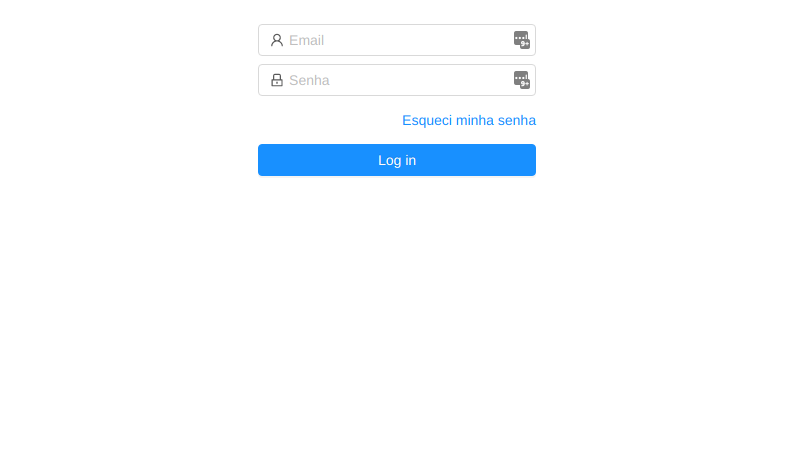
\includegraphics[width=1\textwidth]{figs/tccExtract/login.png}
% \footnotesize Fonte: Autoria Própria
% \end{figure}

Ao acessar a aplicação a tela de login é apresentada, e todas as funcionalidades de usuário da API estão conectadas a tal. Esta tela representa por onde o colegiado deve acessar o sistema.

Após efetuar o login, o usuário deve cadastrar os parâmetros de extração. Como pode ser visto na \textbf{Figura \ref{params}}, é apresentada a tela para cadastro de parâmetros em página específica, e na \textbf{Figura \ref{params2}} para parâmetros de página indefinida. Ao enviar o formulário, o objeto JSON é montado e a RegEx codificada para base64 e assim o cadastro é realizado. Como resultado das informações preenchidas na \textbf{Figura \ref{params}} é apresentado o objeto JSON da \textbf{Figura \ref{jsonParams}}.

\begin{figure}[H]
  \centering
  \caption{Registro de Parâmetro - Sistema de Extração de dados de TCC}
  \subfloat[Registro de Parâmetro de Página Específica]{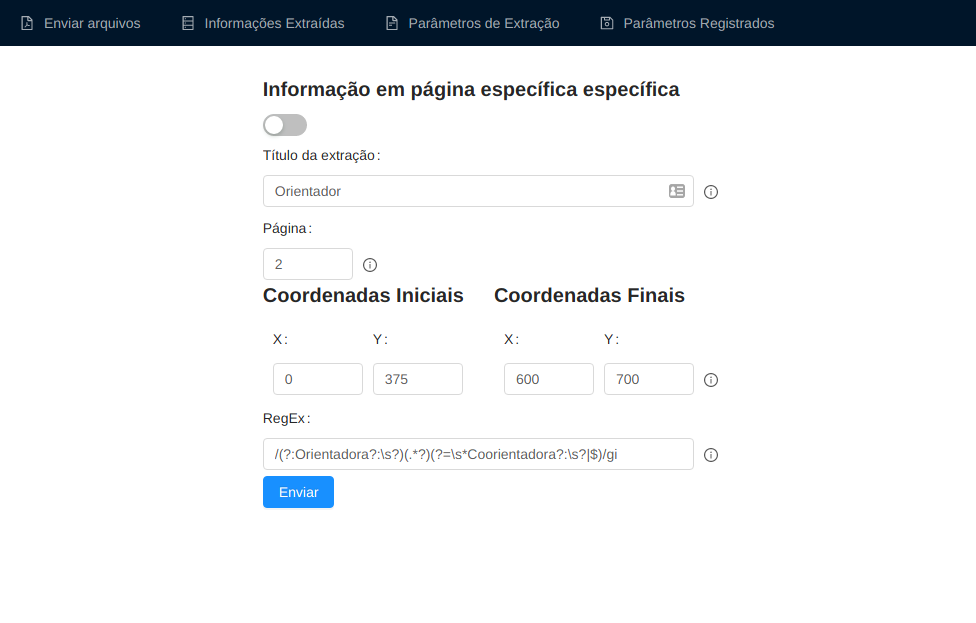
\includegraphics[width=\textwidth]{figs/tccExtract/params.png}\label{params}}
  \hfill
  \subfloat[Registro de Parâmetro de Página Indefinida]{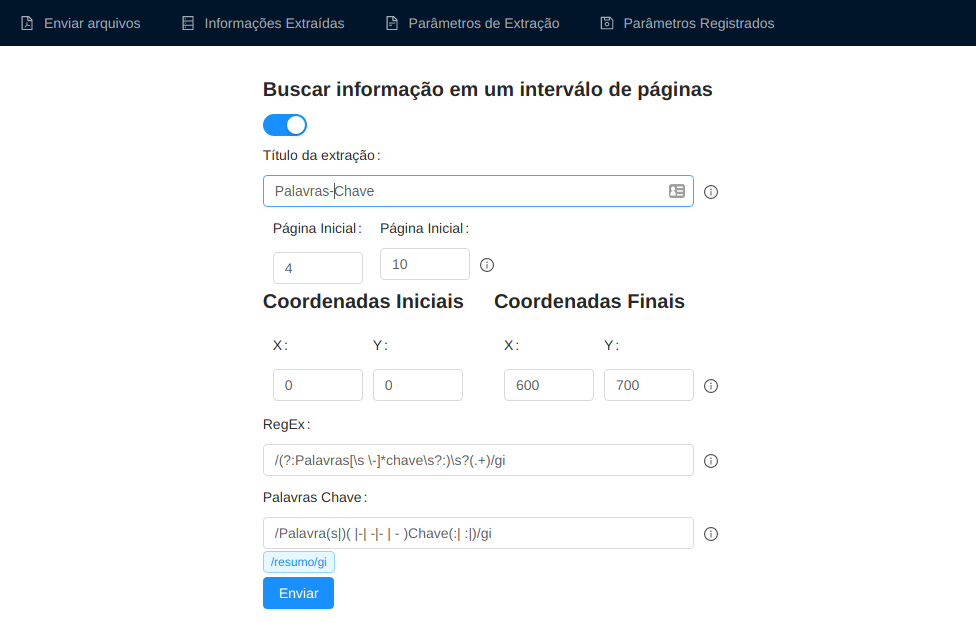
\includegraphics[width=\textwidth]{figs/tccExtract/params2.png}\label{params2}}

\end{figure}

\begin{figure}[H]
\centering
\captionsetup{justification   = raggedright,
              singlelinecheck = false}
\caption{Objeto JSON Resultante do Formulário de Parâmetros de Extração - Sistema de Extração de dados de TCC}\label{jsonParams}
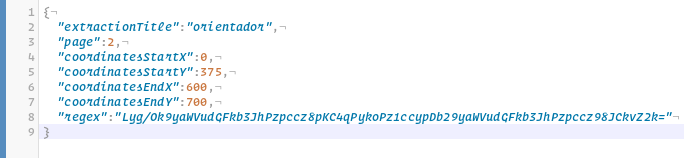
\includegraphics[width=1\textwidth]{figs/jsonParams.png}
\footnotesize Fonte: Autoria Própria
\end{figure}

% \begin{figure}[H]
% \centering
% \captionsetup{justification   = raggedright,
%               singlelinecheck = false}
% \caption{Registro de Parâmetro de Página Específica - Sistema de Extração de dados de TCC}\label{params}
% 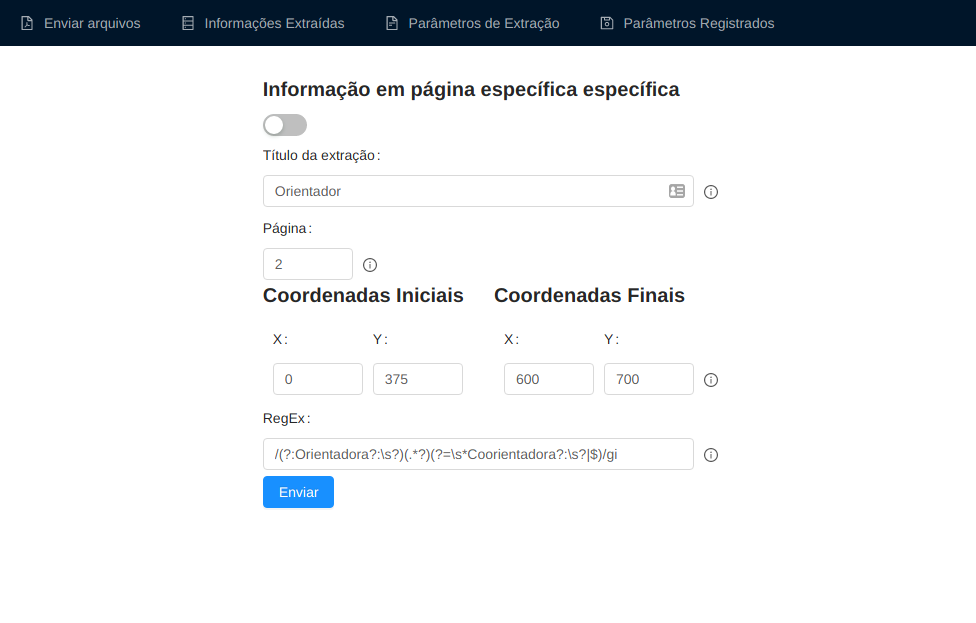
\includegraphics[width=1\textwidth]{figs/tccExtract/params.png}
% \footnotesize Fonte: Autoria Própria
% \end{figure}

% \begin{figure}[H]
% \centering
% \captionsetup{justification   = raggedright,
%               singlelinecheck = false}
% \caption{Registro de Parâmetro de Página Indefinida - Sistema de Extração de dados de TCC}\label{params2}
% 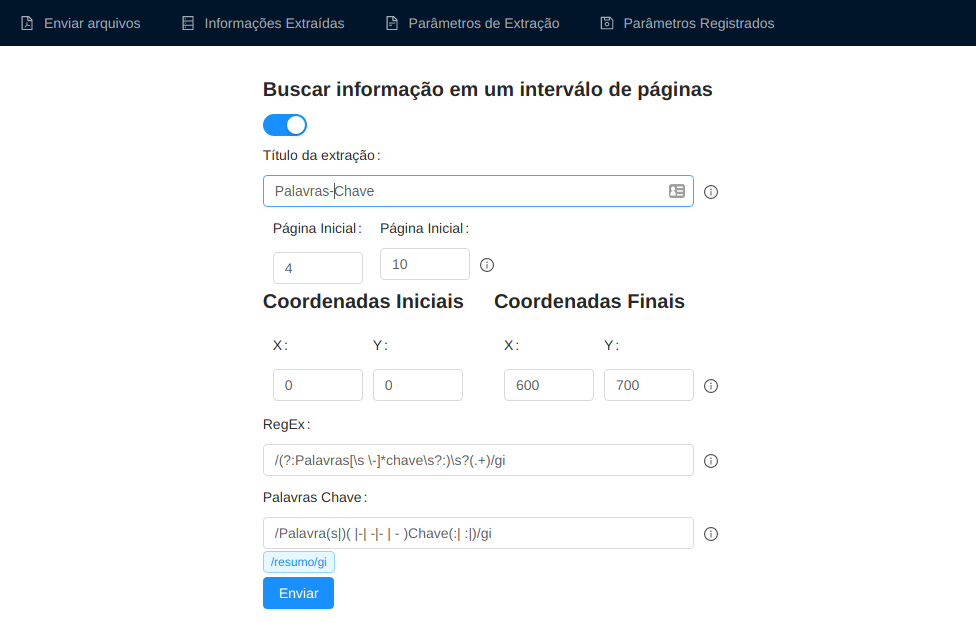
\includegraphics[width=1\textwidth]{figs/tccExtract/params2.png}
% \footnotesize Fonte: Autoria Própria
% \end{figure}

Os parâmetros registrados podem ser consultados na próxima aba, como apresentado na \textbf{Figura \ref{paramsR}}, lá a informação é recuperada do banco de dados e é possível remover um registro, caso desejado.

\begin{figure}[H]
\centering
\captionsetup{justification   = raggedright,
              singlelinecheck = false}
\caption{Parâmetros Registrados - Sistema de Extração de dados de TCC}\label{paramsR}
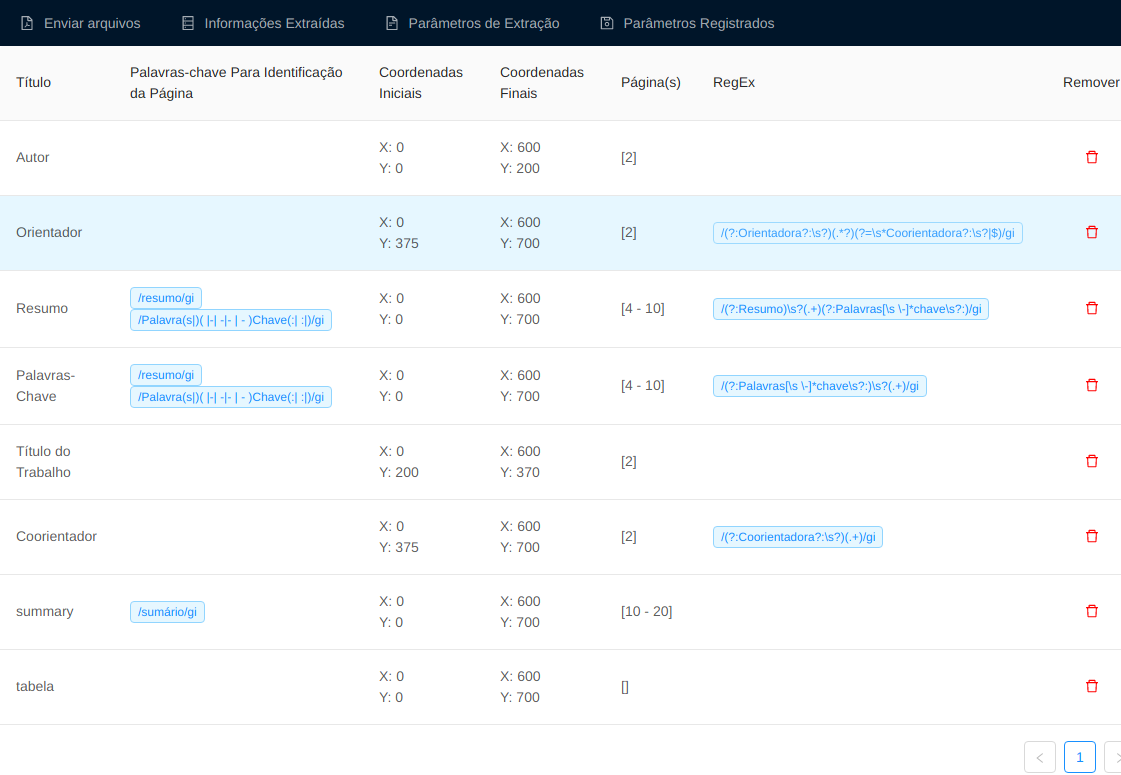
\includegraphics[width=1\textwidth]{figs/tccExtract/paramsR2.png}
\footnotesize Fonte: Autoria Própria
\end{figure}

Com os parâmetros devidamente registrados, é possível submeter novos arquivos, na \textbf{Figura \ref{upload}} o botão de upload apresentado aceita um ou mais arquivos PDF, mas respeitando uma das constrições de API RESTful, é feita apenas uma requisição para cada arquivo.

\begin{figure}[H]
\centering
\captionsetup{justification   = raggedright,
              singlelinecheck = false}
\caption{Envio de Arquivos - Sistema de Extração de dados de TCC}\label{upload}
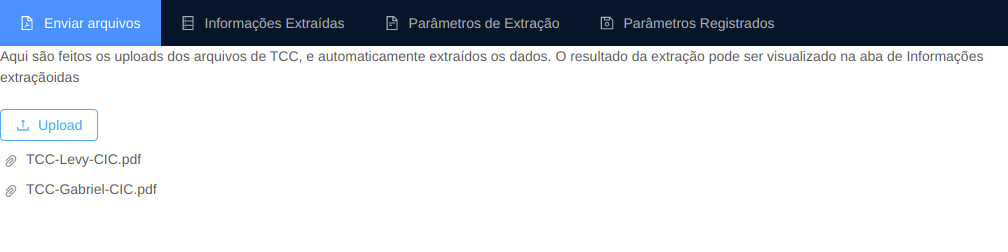
\includegraphics[width=1\textwidth]{figs/tccExtract/upload.png}
\footnotesize Fonte: Autoria Própria
\end{figure}

Após enviado, o resultado da extração pode ser consultado na aba seguinte. A tabela apresentada na \textbf{Figura \ref{extr}} é montada de acordo com os parâmetros que foram definidos como primordiais para o projeto de egressos.

Havendo mais informações extraídas, estas podem ser acessadas no formato de objeto JSON através do botão \textit{Mais} a direita. E o resumo no botão presente à esquerda.

\begin{figure}[H]
\centering
\captionsetup{justification   = raggedright,
              singlelinecheck = false}
\caption{Informações Extraídas - Sistema de Extração de dados de TCC}\label{extr}
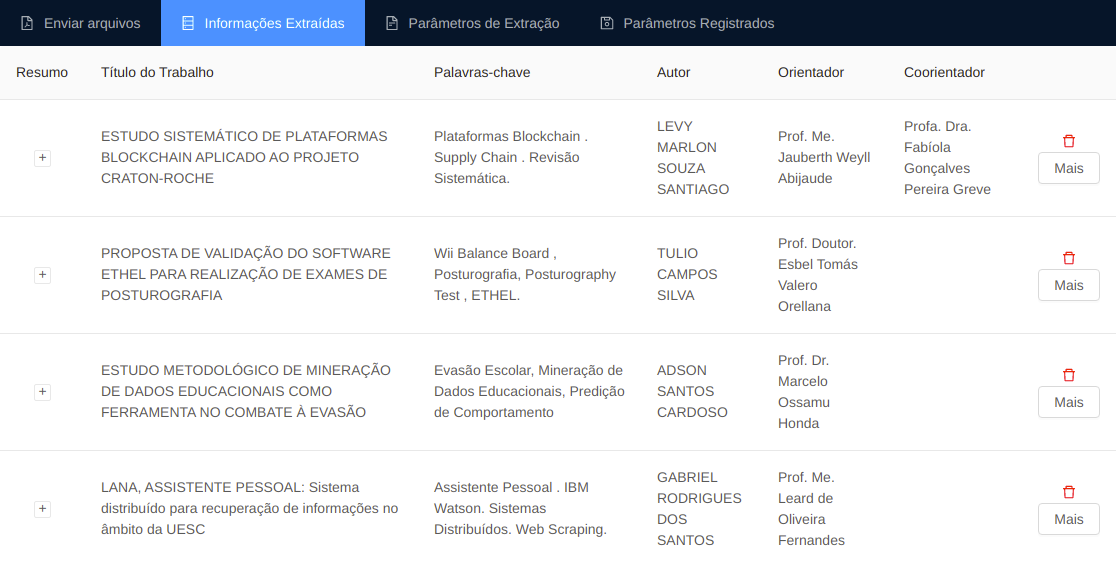
\includegraphics[width=1\textwidth]{figs/tccExtract/extr.png}
\footnotesize Fonte: Autoria Própria
\end{figure}